\chapter{Analisi dei Dati}\label{iTerremotiInItalia}
Questo Capitolo riguarda il lavoro da me svolto, dopo una descrizione dettagliata del cosa voglio fare e come lo voglio fare vado a mettere in pratica quanto detto, entrando nei dettagli del mio lavoro di Tesi. In questo Capitolo spiegher\`o come ho cercato di rispondere alle domande che mi sono posto, sfruttando gli strumenti appresi durante questi anni di studio, ovvero la Programmazione, la Logica Matematica, la Matematica e il Calcolo delle Probabilit\`a; questi mi hanno quindi permesso di creare due applicativi basati su approcci differenti, che vanno sostanzialmente a eseguire operazioni sui dati messi a disposizione dai cataloghi online e vanno a restituire in output due stime, una mirata alla probabilit\`a che avvenga un terremoto ed una mirata alla previsione dei terremoti.\\
La sezione che si occupa di terremoti dell'Istituto Nazionale di Geofisica e Vulcanologia, mette a disposizione online e scaricabile gratuitamente il CPTI15\footnote{Catalogo Parametrico dei Terremoti Italiani, versione 2.0.} \cite{CPTI15} contenente i dati storici registrati dagli strumenti raccolti negli anni dal 1000 al 2017. Il mio obiettivo \`e andare a manipolare questa banca dati resa disponibile, utilizzando algoritmi coerenti che mirino a prevedere e stimare il rischio sismico in determinate aree del paese preso in considerazione.

\section{Approccio generale e dettagli implementativi}\label{dettagliImpl}

Come visto nella Sezione precedente (vedi Sezione \ref{analisiDati}) la rappresentazione dei dati \`e un fattore molto importante per dare un senso agli stessi, pertanto di seguito spiego come ho deciso di rappresentare i dati che ho a disposizione per l'analisi dei terremoti.\\
La migliore visualizzazione che mi \`e venuta in mente per rappresentare dati di terremoti, ma soprattutto per approcciare al tema della previsione e del fattore di rischio, \`e attraverso l'utilizzo di una mappa. Ho quindi strutturato un programma che prende in input le Latitudini e Longitudini di due punti, che andranno a definire rispettivamente: il punto in basso a sinistra e il punto in alto a destra, che collegati opportunamente con 4 linee, ognuna con un estremo in uno dei punti e parallele a 2 a 2, andranno a tracciare un quadrilatero con lati uguali a 2 a 2 (quindi un quadrato o un rettangolo) sulla mappa stessa. Questa area delimitata dalla forma geometrica che ne viene fuori, rappresenta l'insieme dei dati che andremo ad analizzare, pertanto ho impostato il programma in modo che scarti automaticamente i dati contenuti nel file .csv che non rientrano in quest'area. Quindi per maggiore chiarezza faccio un esempio pratico:\\ ho a disposizione 500.000 record nel file in input, ma soltanto 200.000 rientrano nell'area delimitata dalla forma geometrica che ho creato, quindi il programma scarta a priori i 300.000 inutili alla mia analisi, cos\`i da rendere pi\`u veloci eventuali operazioni ed algoritmi che andranno ad operare sui dati.\\
Una volta decisa l'area geografica, l'utilizzatore dovr\`a inserire un intero n, questo servir\`a a suddividere il rettangolo preso inizialmente in considerazione in una griglia (o matrice) costituita da nxn celle. Ci\`o permetter\`a quindi all'utilizzatore di entrare pi\`u nel dettaglio usando un intero n grande, mentre rimanere su una visione pi\`u generale usando un intero n piccolo. Questa \`e una visione del funzionamento di base del programma, di seguito spiego i due approcci che ho utilizzato per rispondere alle due domande che mi sono posto inizialmente.

\subsection{Rischio sismico}\label{rischioSismico}

Il primo approccio che chiamer\`o \textit{``Rischio sismico''} mira ad analizzare i dati con un criterio che permette di rispondere alla domanda:\\
Quanto \`e rischiosa una determinata cella rappresentante un'area geografica rispetto alle altre?\\
Per fare questo ho agito con un criterio logico descritto di seguito. Come spiegato nella sezione precedente (vedi Sezione \ref{dettagliImpl}) ho a disposizione un'area delimitata da una griglia nxn. Inizialmente ho preso in considerazione gli eventi sismici del CPTI15, che sono poco meno di 5000 record, per cominciare a strutturare l'algoritmo per analizzare i dati (naturalmente questo primo database che ho utilizzato non permette una Big Data analytics, questo perch\`e i record contenuti sono relativamente pochi, ma una volta definito l'approccio e testato il funzionamento, il programma potr\`a prendere in maniera dinamica i dati, non sar\`a quindi un problema analizzare cataloghi con una mole di dati tale da poter essere definita una Big Data analytics). L'obiettivo che mi sono posto \`e quello di andare a colorare ogni cella della griglia in base alla somma delle magnitudo avvenute nelle rispettive celle. Per fare questo ho utilizzato tre colori, il verde, il giallo ed il rosso; sono andato poi anche a sfruttare l'opacit\`a del colore per avere una scala pi\`u dettagliata senza utilizzare pi\`u di tre colori. Quindi una volta completato l'algoritmo l'output che otterr\`o sar\`a una mappa dell'Italia, con una griglia nxn dove ogni cella ha un colore; se la cella ha un fattore di rischio basso, sar\`a colorata di verde chiaro, se ha un fattore di rischio alto sar\`a colorata di un rosso pi\`u scuro.\\
Ora vado ad analizzare nel dettaglio il criterio che permette di stabilire il fattore di rischio, che verr\`a utilizzato per colorare le celle della mappa.\\
Presa la matrice che rappresenta la griglia avente nxn celle, scorro i dati che sono memorizzati nel file .csv in ordine cronologico non decrescente (condizione necessaria, utile pi\`u tardi nel secondo approccio), quindi per ogni record se il terremoto \`e avvenuto nella cella i-esima incremento il valore della cella del valore della magnitudo del terremoto i-esimo, pertanto alla fine avr\`o una matrice contenente in ogni cella la somma delle magnitudo dei terremoti che si sono verificati dentro quella cella. A questo punto sommo il valore di tutte le celle, ed avr\`o la somma complessiva delle magnitudo dei terremoti avvenuti in tutte le celle, ora dividendo il valore di ogni cella per questa somma ottenuta e sostituendolo al valore precedente che aveva ogni cella, avr\`o una matrice che somma a 1.\\
Per colorare la mappa in maniera dinamica, ho deciso di stabilire un fattore di rischio che va da 0.0 a 100.0, quindi prendere il valore massimo contenuto tra tutte le celle ed assegnargli un fattore di rischio di 100.0 su 100.0. Questo comporter\`a che per ogni possibile n scelto in input, ci sar\`a sempre una cella con fattore di rischio massimo e tutte le altre saranno colorate di conseguenza in output. La colorazione sar\`a rapportata al fattore di rischio nel seguente modo:
\begin{itemize}
\item Fattore di rischio $\le$ 10 colore verde opacit\`a 30\%
\item Fattore di rischio $>$ 10 e $\le$ 20 colore giallo opacit\`a 30\%
\item Fattore di rischio $>$ 20 e $\le$ 30 colore giallo opacit\`a 40\%
\item Fattore di rischio $>$ 30 e $\le$ 40 colore giallo opacit\`a 50\%
\item Fattore di rischio $>$ 40 e $\le$ 50 colore rosso opacit\`a 30\%
\item Fattore di rischio $>$ 50 e $\le$ 70 colore rosso opacit\`a 40\%
\item Fattore di rischio $>$ 70 colore rosso opacit\`a 60\%
\end{itemize}

\subsubsection{Risultati}

Di seguito vediamo una serie di test effettuati lanciando il primo programma che si basa sull'approccio \textit{``Rischio sismico''}:

\begin{figure}[H]
   \centering
   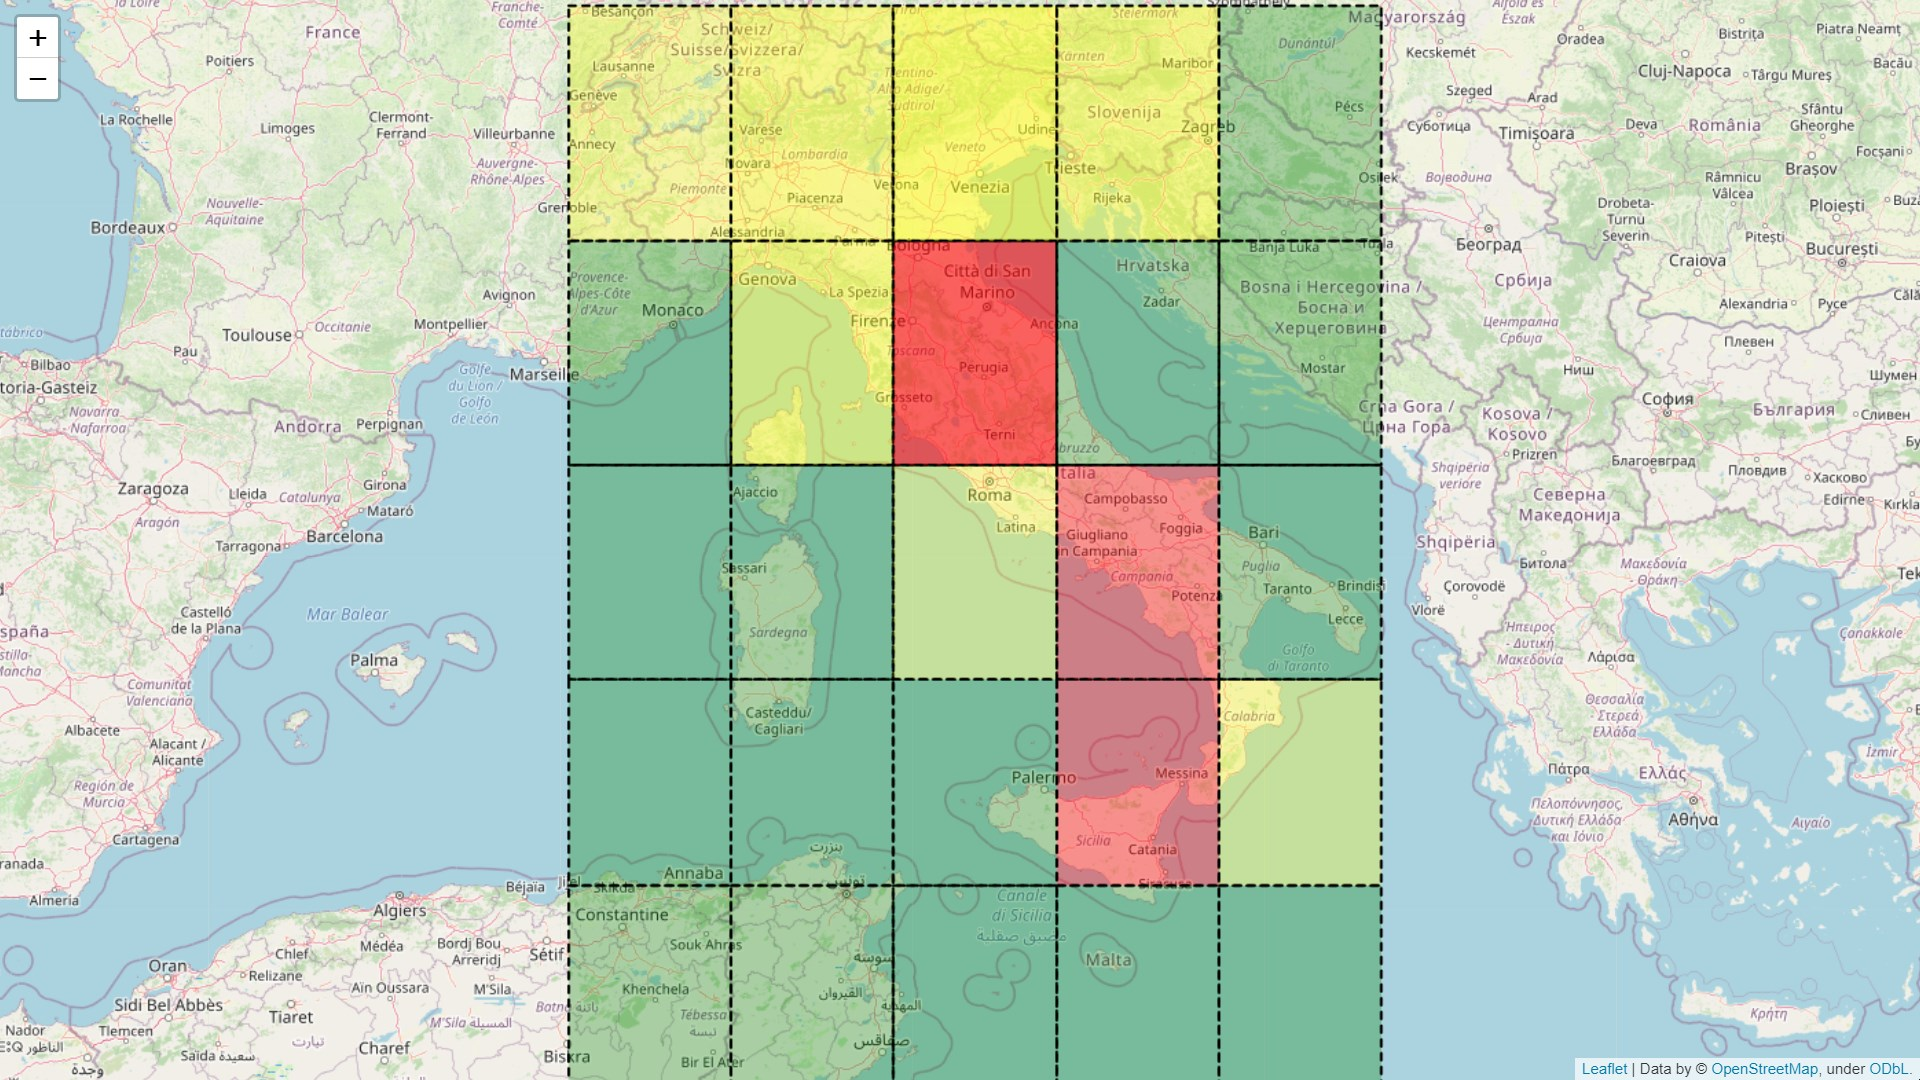
\includegraphics[width=0.835\textwidth]{images/5x5_CPTI15.jpg}
   \caption{Griglia 5x5 con DB CPTI15}
\end{figure}

Questo \`e l'output del programma se lanciato prendendo in considerazione l'Italia, con la base dati CPTI15, e con n=5. Come si evidenzia abbiamo una cella con fattore di rischio 100 che \`e quella posizionata nel centro Italia e le altre che si basano su quella come riferimento, quindi le due con fattore di rischio, subito precedenti al massimo sono le due che vediamo nella zona del meridione e tra Calabria e Sicilia.

\begin{figure}[H]
   \centering
   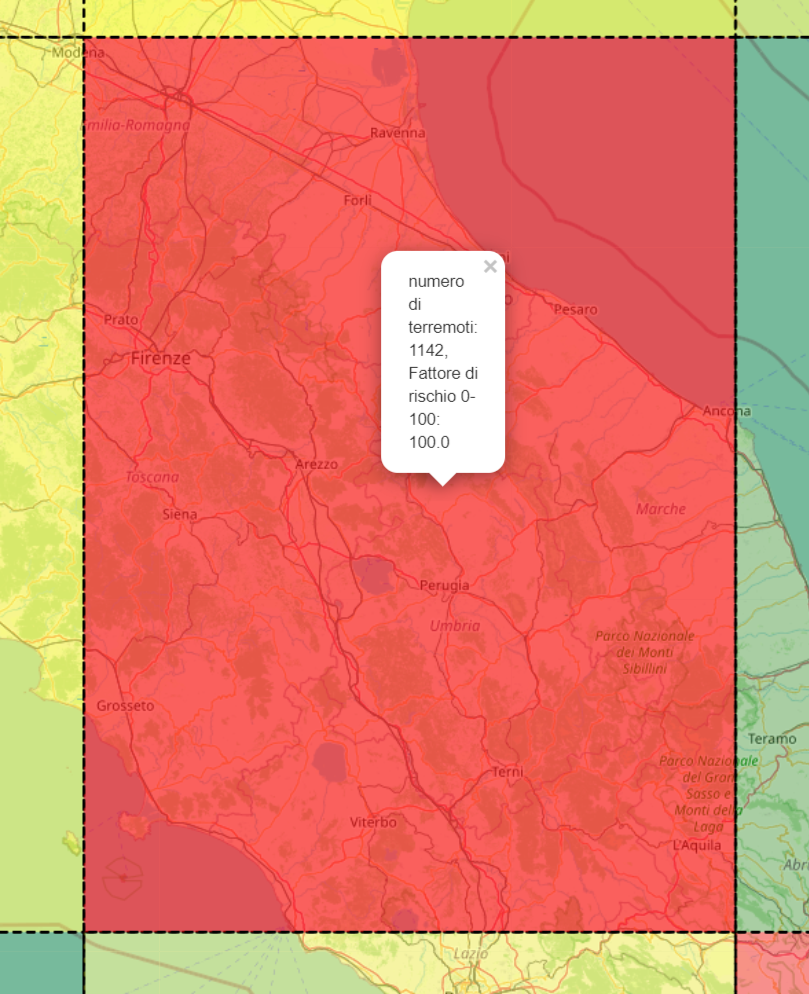
\includegraphics[width=0.600\textwidth]{images/FattoreDiRischio5x5_CPTI15_centro.png}
   \caption{Griglia 5x5 con DB CPTI15, zoom dettaglio centro Italia}
   \label{fig:zonaCentrale}
\end{figure}

\begin{figure}[H]
   \centering
   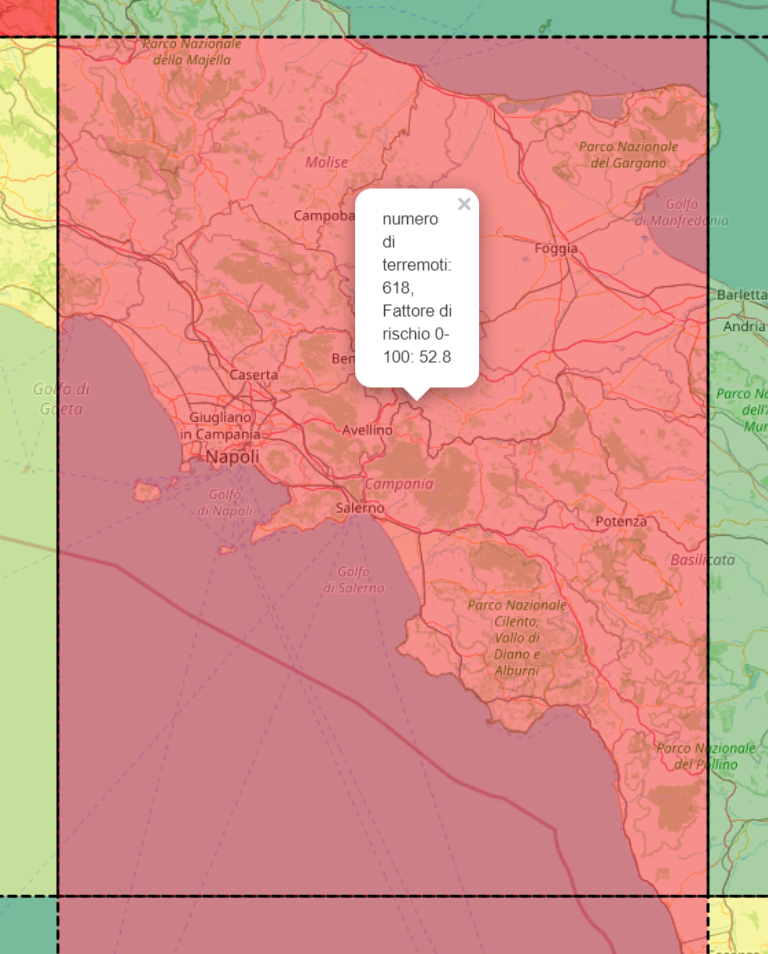
\includegraphics[width=0.600\textwidth]{images/FattoreDiRischio5x5_CPTI15_meridione.png}
   \caption{Griglia 5x5 con DB CPTI15, zoom dettaglio Italia meridionale}
   \label{fig:zonaMeridionale}
\end{figure}

Di seguito ci sono altri due esempi di come il programma permette di entrare pi\`u nel dettaglio, andando ad analizzare due casi specifici, nella Figura \ref{fig:zonaCentrale} possiamo vedere un pop-up sulla cella relativa alla zona centrale, con fattore di rischio maggiore, che ci dir\`a quanti terremoti sono avvenuti in questa cella e il relativo fattore di rischio. Nella successiva Figura \ref{fig:zonaMeridionale} possiamo vedere come il fattore di rischio sia poco pi\`u della met\`a rispetto al massimo, quindi avremo la cella colorata di rosso con un'opacit\`a del 40\%.

\begin{figure}[H]
   \centering
   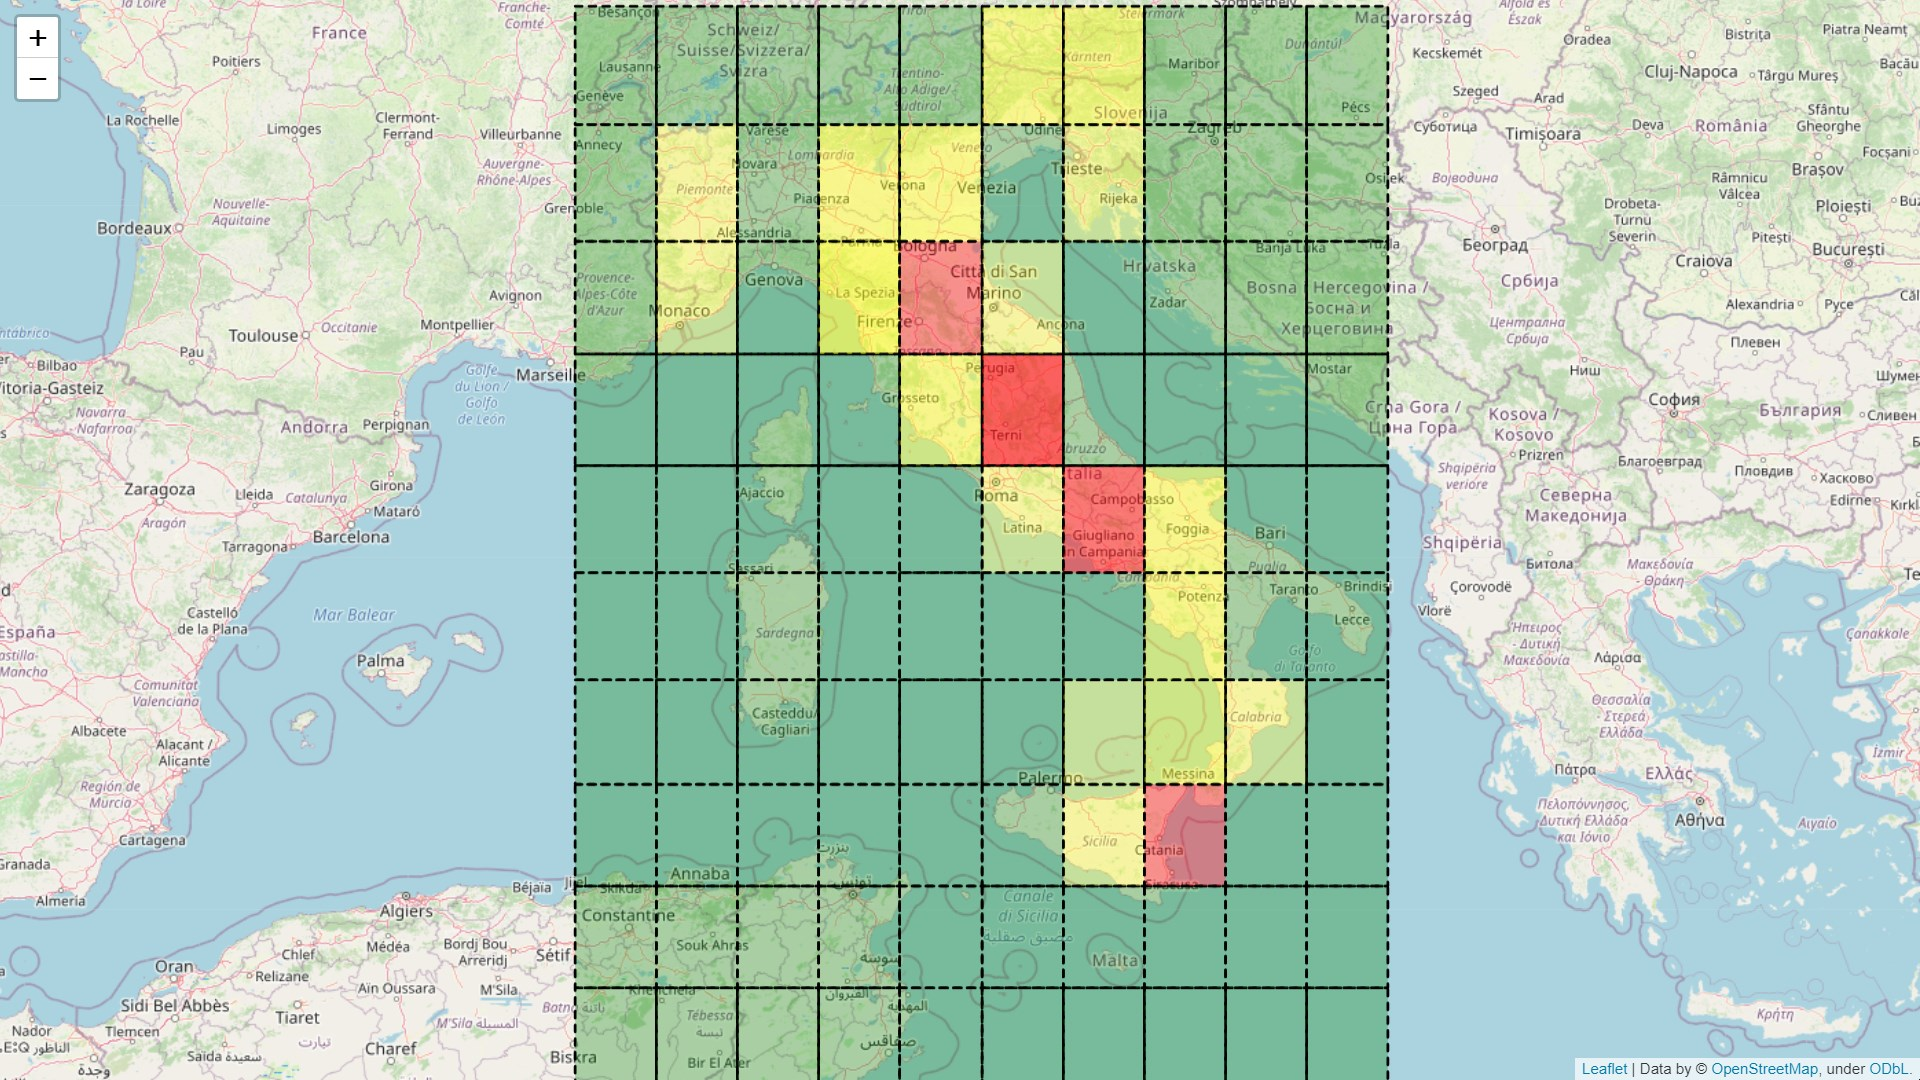
\includegraphics[width=0.835\textwidth]{images/10x10_CPTI15.jpg}
   \caption{Griglia 10x10 con DB CPTI15}
   \label{fig:10x10CPTI15}
\end{figure}

\begin{figure}[H]
   \centering
   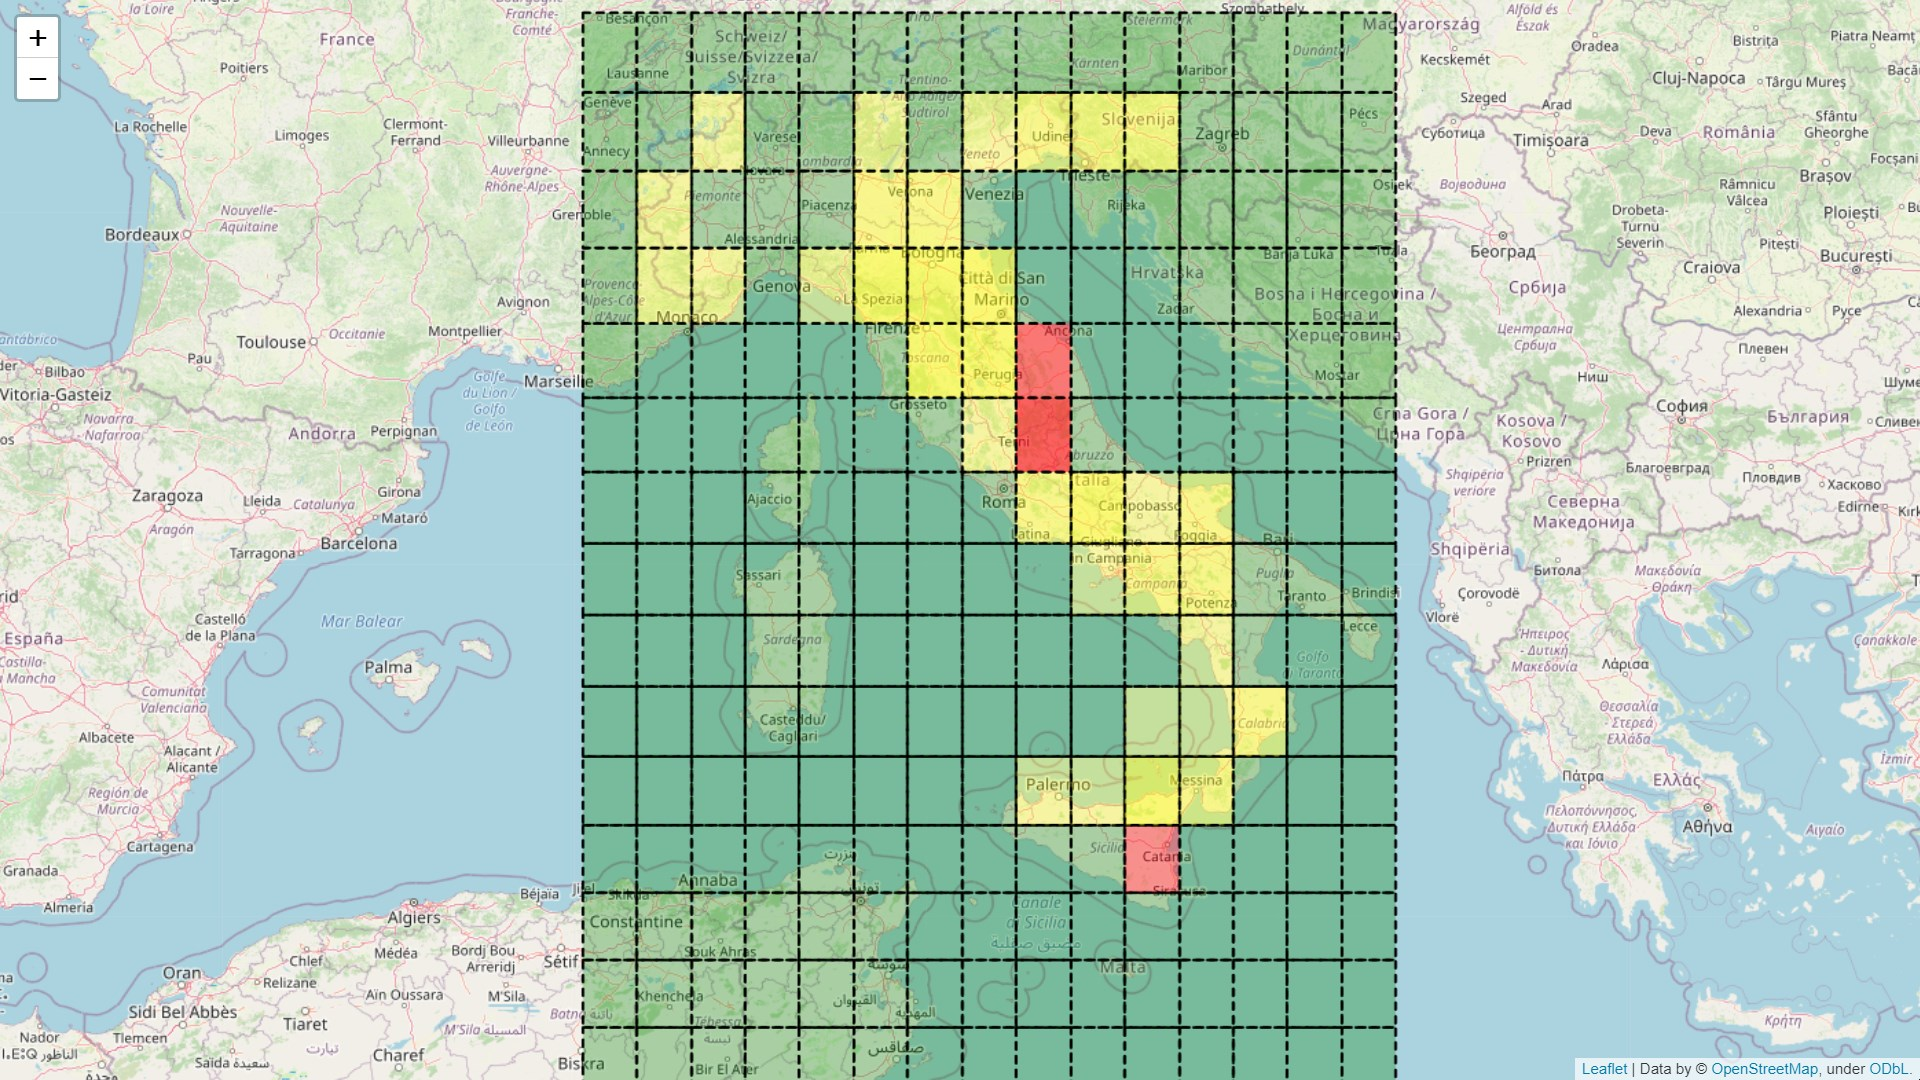
\includegraphics[width=0.835\textwidth]{images/15x15_CPTI15.jpg}
   \caption{Griglia 15x15 con DB CPTI15}
   \label{fig:15x15CPTI15}
\end{figure}

Nelle Figure \ref{fig:10x10CPTI15} e \ref{fig:15x15CPTI15} sopra vediamo come cambiando la n in input, rispettivamente in 10 e 15, otteniamo due griglie aventi rispettivamente 100 celle e 225 celle. Questo permette di fare un analisi pi\`u dettagliata restringendo cos\`i l'area ricoperta da ogni cella.

\begin{figure}[H]
   \centering
   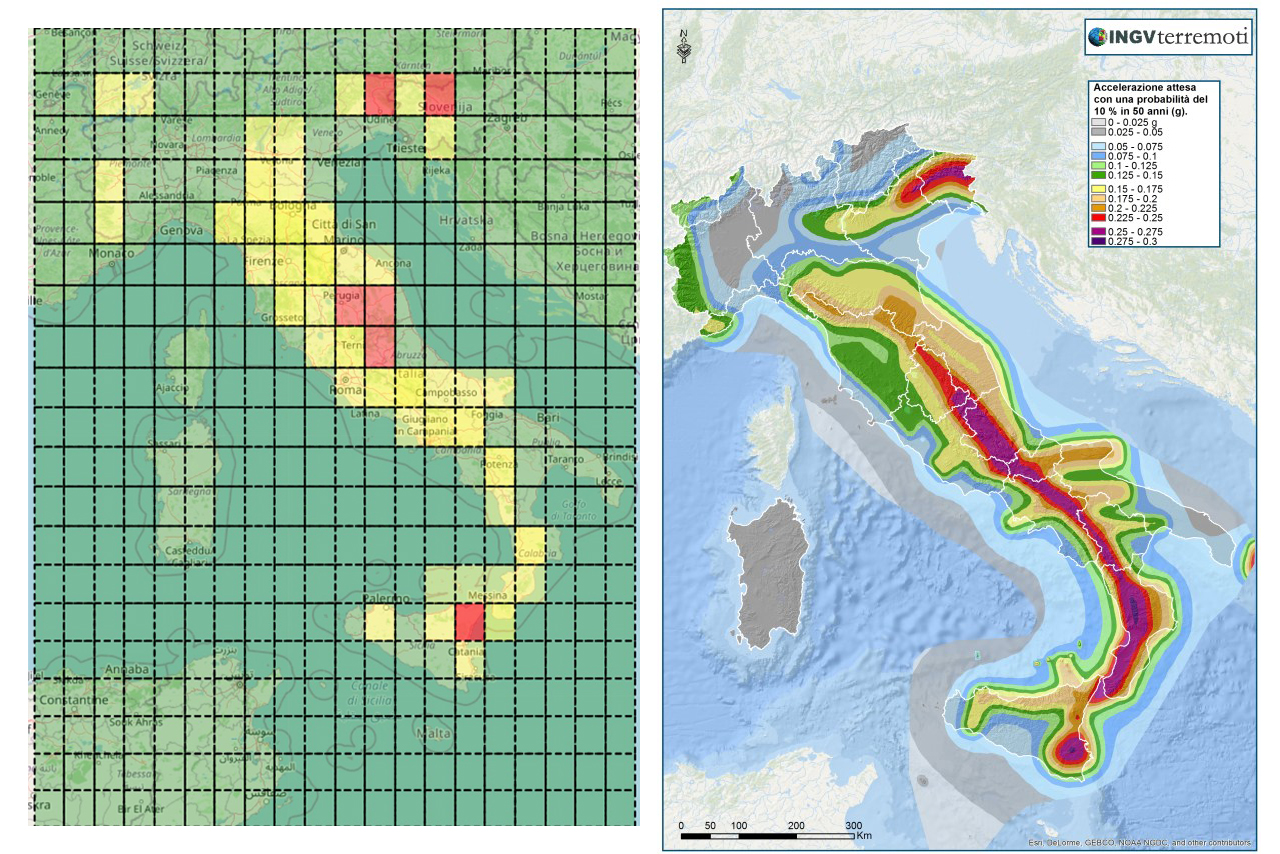
\includegraphics[width=0.835\textwidth]{images/mappaPericolositaVs20x20.jpg}
   \caption{Confronto griglia 20x20 con mappa pericolosit\`a sismica del territorio nazionale}
   \label{fig:20x20vsWarningMap}
\end{figure}

Ora ho voluto prendere in considerazione l'output del programma con n=20 come input, avendo cos\`i ristretto ancor di pi\`u l'area di ogni cella. Ho quindi messo a confronto la griglia di 400 celle con la mappa di pericolosit\`a sismica del territorio nazionale vista in precedenza (vedi Figura \ref{img:mappaPericolo}), questo porta alla luce come gi\`a l'approccio pi\`u logico, ovvero la somma delle magnitudo degli eventi sismici avvenuti in ogni cella dia un risultato molto vicino alla mappa di pericolosit\`a sismica attualmente pubblicata dall'INGV. Come detto in precedenza questo programma non tiene in considerazione precursori sismici, bens\'i si basa solo ed esclusivamente sull'analisi dei dati storici a disposizione. L'analisi appena fatta non permette di poter affermare nulla, se non che nelle celle rosse in passato sono avvenuti pi\`u eventi sismici o comunque eventi sismici di maggiore entit\`a rispetto le altre. Ora per provare il programma e testarne il comportamento con una mole di dati superiore andr\`o ad utilizzare il database messo a disposizione dell'USGS\footnote{Agenzia scientifica del Governo degli Stati Uniti, suddivisa in dipartimenti che si occupano delle seguenti aree scientifiche: biologia, geografia, geologia e idrologia} (United States Geological Survey - Agenzia per la Sorveglianza Geologica degli Stati Uniti), contenente 1.800.000 eventi sismici, dei quali circa 21.000 avvenuti nel territorio italiano, negli anni 1960-2017.

\begin{figure}[H]
   \centering
   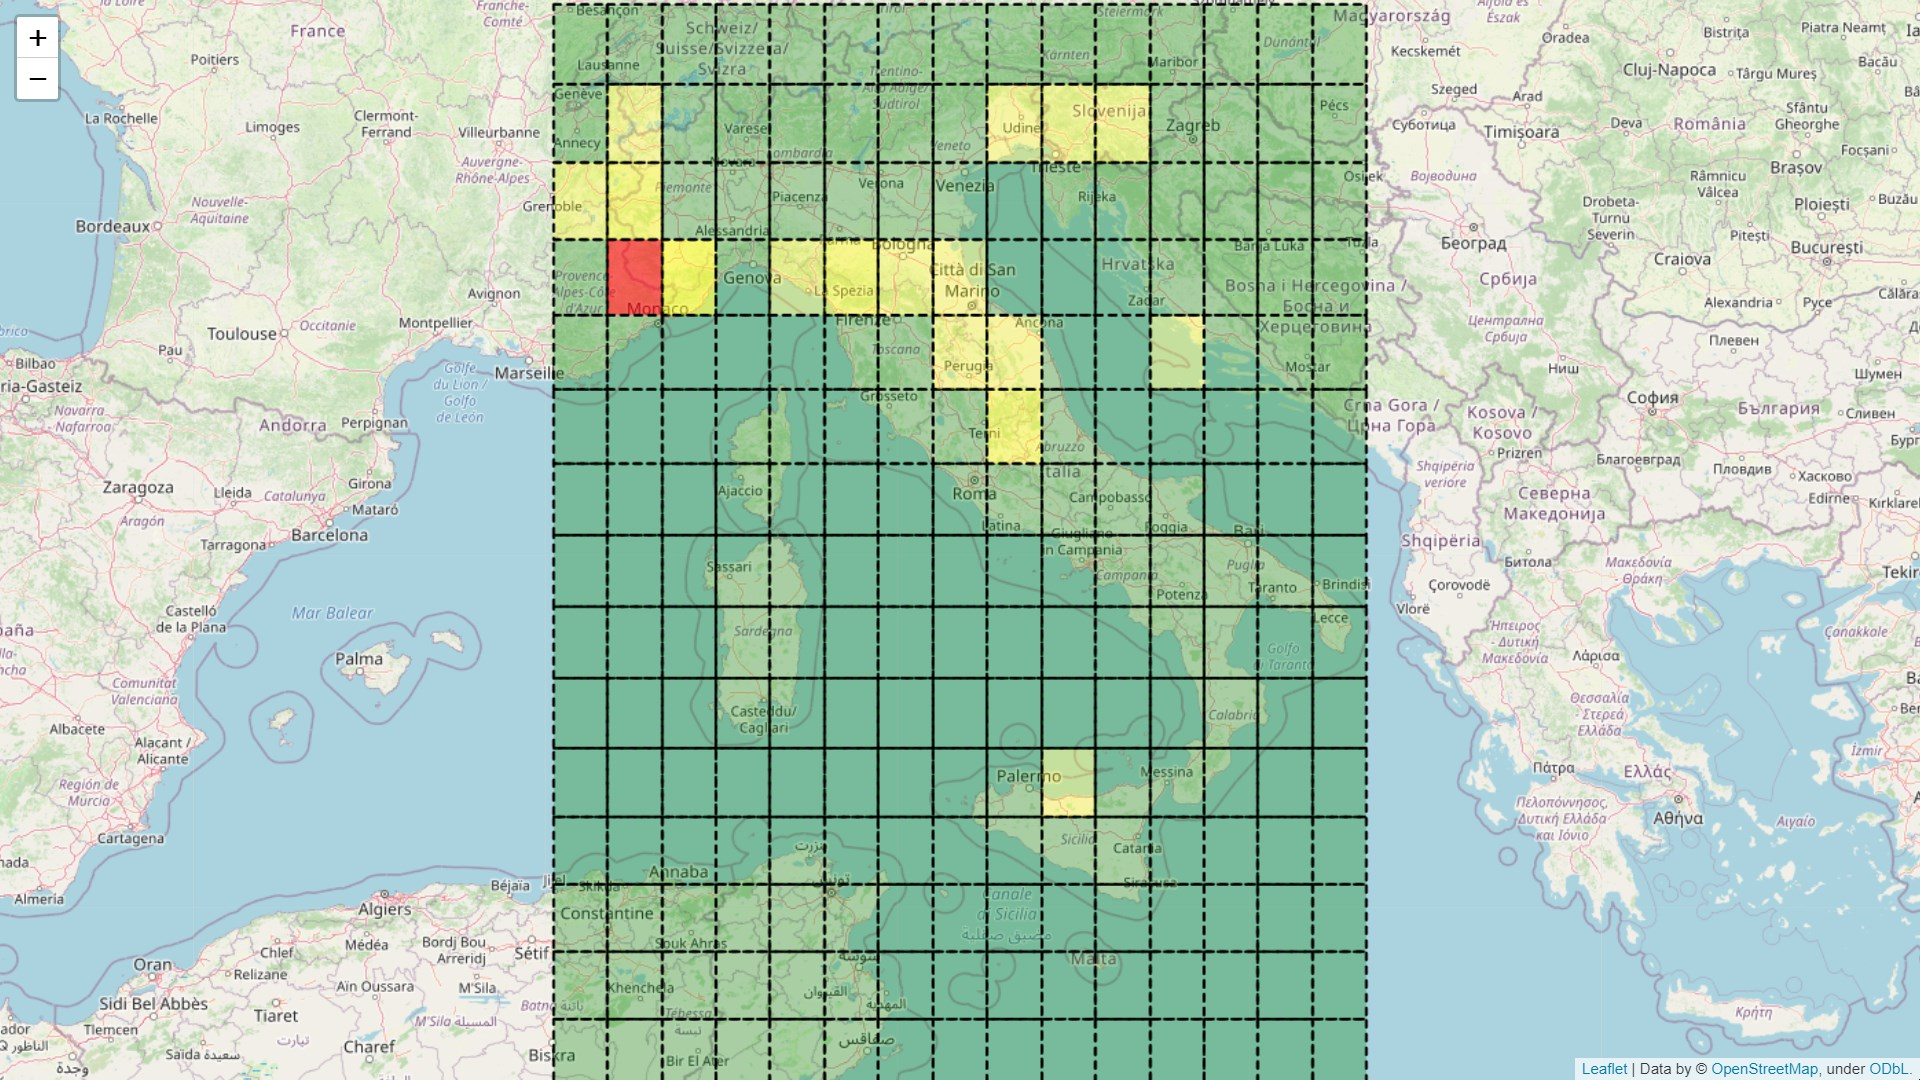
\includegraphics[width=0.835\textwidth]{images/15x15_USGS.jpg}
   \caption{Griglia 15x15 con DB USGS}
   \label{fig:15x15USGS}
\end{figure}

\begin{figure}[H]
   \centering
   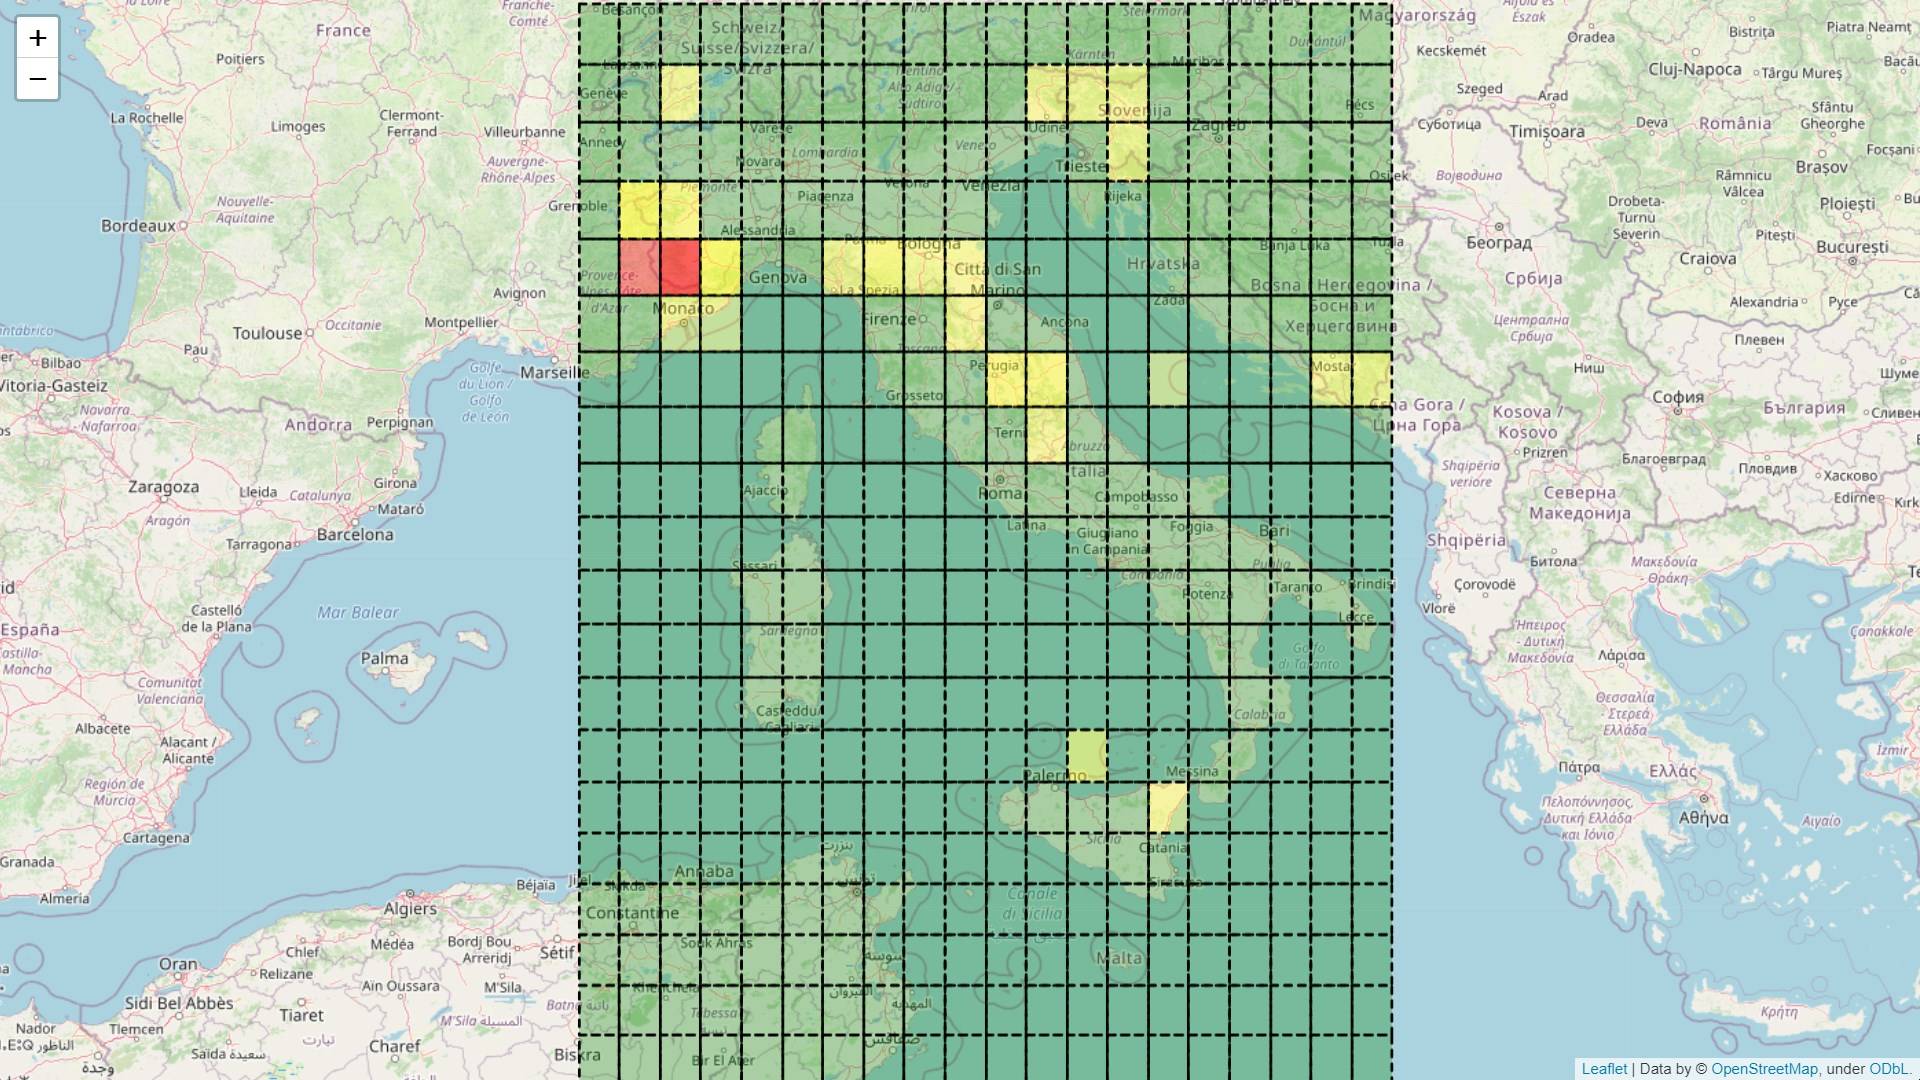
\includegraphics[width=0.835\textwidth]{images/20x20_USGS.jpg}
   \caption{Griglia 20x20 con DB USGS}
   \label{fig:20x20USGS}
\end{figure}

Notiamo subito una differenza grafica tra i dati del CPTI15 e dello USGS. Questo avviene perch\`e le celle vengono confrontate con quella avente fattore di rischio maggiore rispetto alle altre, pertanto nella Figura \ref{fig:15x15USGS} abbiamo 6240 eventi sismici avvenuti tutti nella cella 2x4 mentre nelle altre celle, a partire da quelle colorate di giallo scuro abbiamo dai 2200 eventi in gi\`u. Questo rimane uguale se andiamo ad aumentare la n in input ponendola uguale a 20, infatti la situazione nella Figura \ref{fig:20x20USGS} \`e pressocch\'e simile, se non che la cella con fattore di rischio massimo \`e la 3x5 con 4254 eventi sismici.\\
L'ultimo risultato che voglio portare alla luce \`e il confronto tra le mappe con griglia 20x20 generate dallo USGS e dal CPTI15. Come si vede, le celle precedentemente rosse sulla mappa relativa al CPTI15 sono diventate gialle, perch\'e cambiando la base dati di riferimento \`e cambiata anche la cella di riferimento con fattore di rischio maggiore.

\begin{figure}[H]
   \centering
   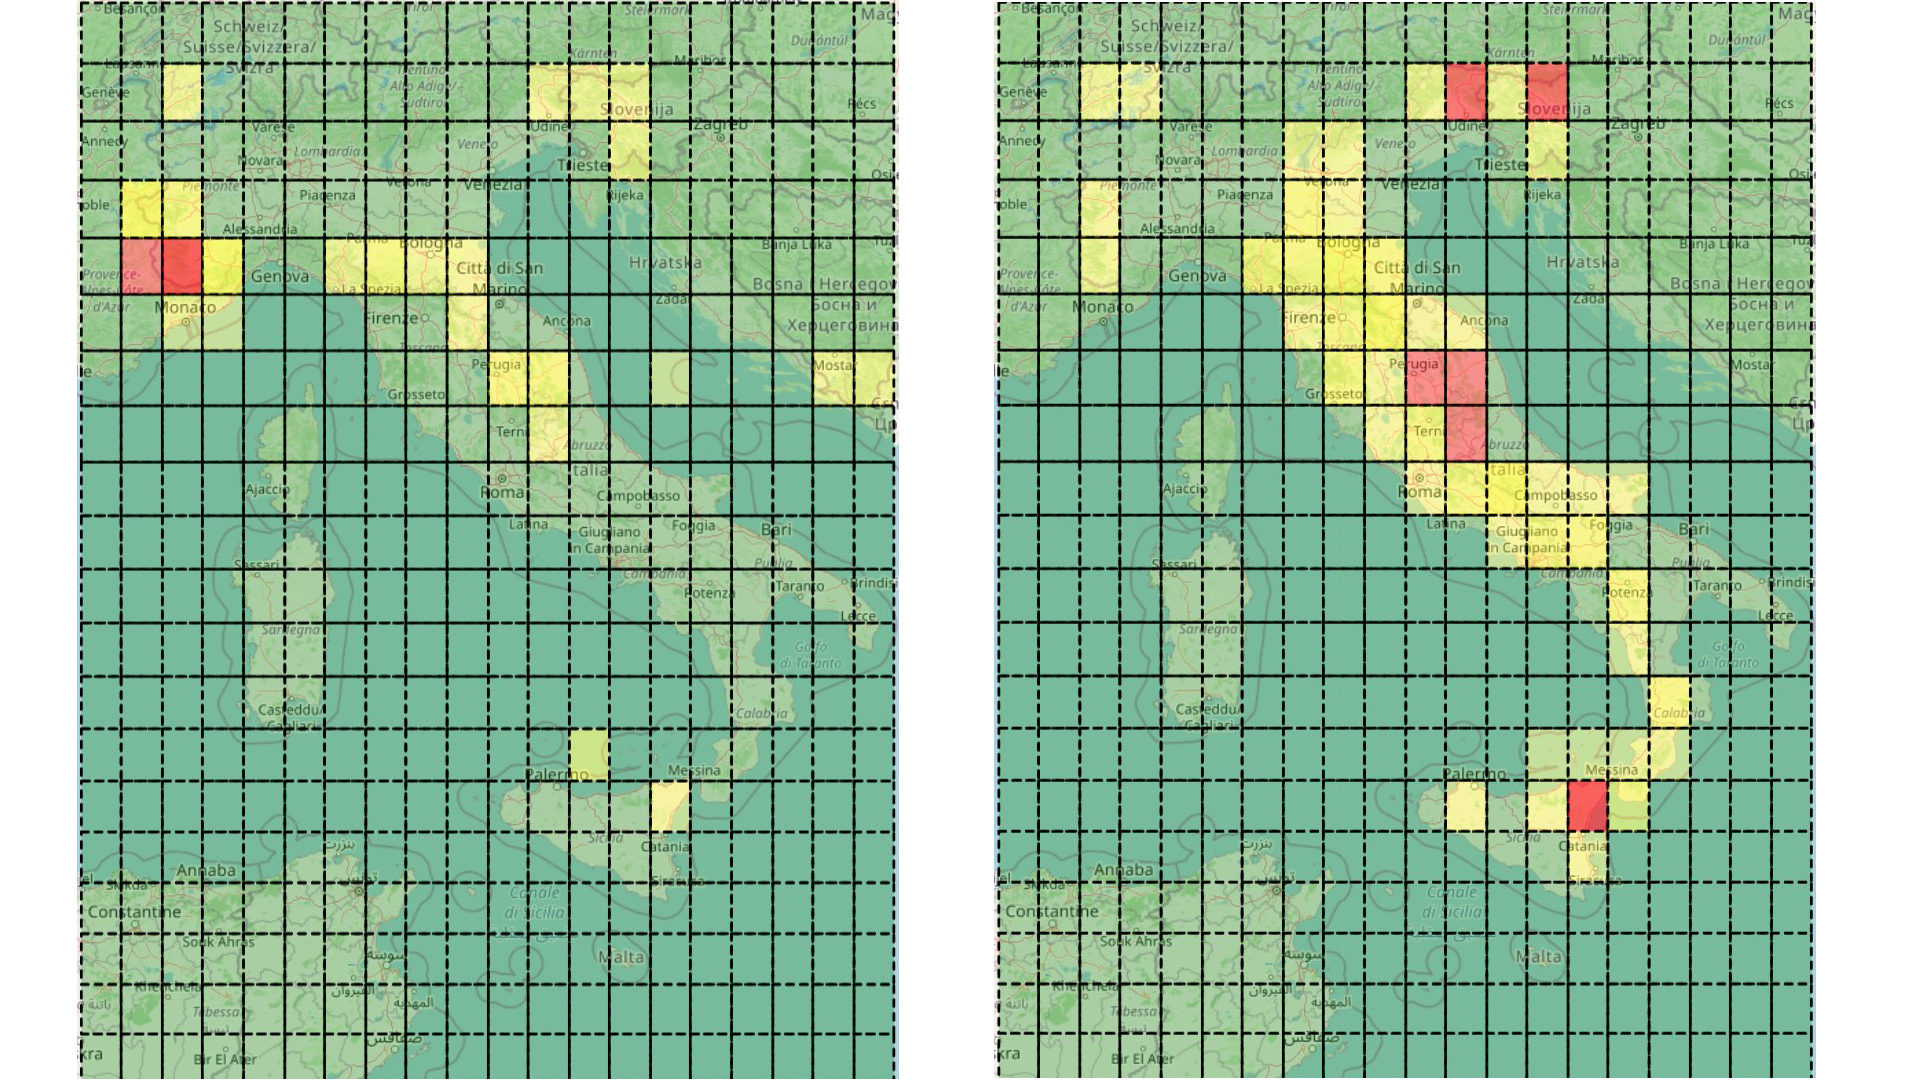
\includegraphics[width=1.0\textwidth]{images/20x20_USGS_vs_CPTI15.jpg}
   \caption{Confronto griglia 20x20 con DB USGS e griglia 20x20 con DB CPTI15}
\end{figure}

\subsection{Previsione}

Il secondo approccio che chiamer\`o \textit{Previsione} mira ad analizzare i dati con un criterio che permette di rispondere alla domanda:\\
Quando avverr\`a il prossimo terremoto con magnitudo maggiore di x, con 0$\le$x$\le$10, nella cella i-esima?\\
Come \`e chiaro dai Capitoli precedenti, la previsione dei terremoti \`e un campo di studio molto ampio e che vede impegnate persone di ogni paese nella ricerca di tecniche predittive, nonostante questo attualmente la previsione si limita a dare delle stime a medio/lungo termine, questo per evidenziare che la domanda alla quale vorrei rispondere attraverso il secondo approccio nasconde insidie nelle quali \`e pericoloso avventurarsi, o meglio, per fare un affermazione che risponda alla domanda dovrei avere una certezza che non mi \`e possibile avere, quindi la domanda che mi pongo con il secondo approccio \`e una domanda che mi fornisce un metodo di analisi e mi permette di produrre un output utilizzando un criterio attendibile, che si avvicina quanto pi\`u possibile alla previsione dei terremoti.\\
Per fare questo vado a prendere in considerazione la griglia nxn che delimita l'area sottoposta ad analisi ed anche in questo caso prendo il CPTI15 descritto ad inizio Capitolo per strutturare il programma. Il criterio che utilizzer\`o avr\`a bisogno, oltre ai dati richiesti nel programma basato sul primo approccio, anche della data nella quale \`e avvenuto il terremoto, quindi ogni record del catalogo che prendiamo in input avr\`a un valore data che dovr\`a necessariamente essere in formato UTC (yyyy-mm-ddTHH:MM:SS.f), ci tengo a precisare che nella maggior parte dei casi, a prescindere dal catalogo preso in considerazione, i dati registrati negli anni passati, diciamo da prima del XX secolo, mancano di alcune informazioni, una di queste \`e l'ora o addirittura il giorno in cui si \`e verificato il terremoto; questa eccezione l'ho gestita settando i dati mancanti a 0, nel caso di ore, minuti e secondi e ad 1 nel caso di giorni e mesi. A prescindere da questa modifica ai dati in input, la mia analisi prender\`a in considerazione soltanto giorno, mese e anno.\\
L'algoritmo calcola tutte le differenze in giorni trascorsi tra un sisma e il successivo (assumo che i dati in input siano ordinati in ordine non decrescente di data, come avviene nei cataloghi pi\`u blasonati messi a disposizione online) per ogni cella, ricordo che prender\`o in considerazione soltanto sismi con una magnitudo maggiore di una certa x che sar\`a data in input. Una volta che ho calcolato tutte le differenze in giorni della cella i-esima mi ricavo la media e la varianza (prender\`o in considerazione soltanto le celle con un numero superiore a 10 di terremoti avvenuti), quindi avr\`o media e varianza di quanto trascorre tra un terremoto ed il successivo, superiori di una certa magnitudo x nella cella i-esima. Per fare questo andr\`o ad utilizzare la Formula \ref{chebyshev} vista nel Background relativo alla disuguaglianza di Chebyshev (vedi Sezione \ref{disuguaglianzaChebyshev}).
Usando quindi le rilevazioni empiriche sul passato e assumendo che l'intervallo di tempo che intercorre fra due terremoti si comporti come una variabile aleatoria, con la disuguaglianza di Chebyshev stimo un intervallo superiore in giorni ($\mu + \lambda\sigma$ tale che $\lambda$ = 2) entro i quali potr\`a avvenire il prossimo terremoto con una probabilit\`a del 75\%.\\
Fatto questo otterr\`o un numero di giorni entro il quale avverr\`a il prossimo terremoto di magnitudo maggiore di x con una probabilit\`a del 75\%, per rendere pi\`u chiaro il risultato lo scriver\`o come anni + giorni, assumendo che l'anno \`e composto da 365 giorni (esempio: 1743 giorni verr\`a restituito in output come 4 anni + 283 giorni).\\
Anche in questo secondo approccio vado ad utilizzare la colorazione, che questa volta \`e basata sui giorni, ovvero la cella colorata di rosso scuro (cella di riferimento) sar\`a quella con il numero di giorni minore rispetto alle altre. I colori sono distribuiti come nell'approccio ``Rischio sismico'' (vedi Sezione \ref{rischioSismico}), pertanto ometto il criterio di colorazione.\\
Questo approccio comporta la verifica di quanto sviluppato per valutarne l'attendibilit\`a, per fare questo ho suddiviso il CPTI15 in due parti approssimativamente uguali in quanto a numero di record, la prima parte prende in considerazione i terremoti avvenuti dal 1000 al 1980, mentre la seconda parte prende in considerazione i terremoti avvenuti dal 1981 al 2017. Arrivato a questo punto quello di cui avevo bisogno era un programma che mi permettesse di verificare se il mio secondo approccio fosse efficiente, ho quindi strutturato un programma che preso in input un catalogo, un anno massimo di riferimento y e la magnitudo minima x, ritorna in output una mappa come quelle dei precedenti approcci spiegati, dove la cella i-esima \`e colorata di verde nel caso in cui sia avvenuto un terremoto dal 1981 al anno y dato in input, prendendo sempre in considerazione soltanto i terremoti con una magnitudo maggiore di x, di nero altrimenti. Inoltre saranno evidenziati su mappa anche i terremoti e in un popup il numero di terremoti avvenuti in ogni cella, cos\'i da poter avere a disposizione pi\`u dati possibili per l'analisi.

\subsubsection{Risultati}

Vado ora ad eseguire una serie di test con analisi annessa del programma che si basa sull'approccio \textit{"Previsione"}

\begin{figure}[H]
   \centering
   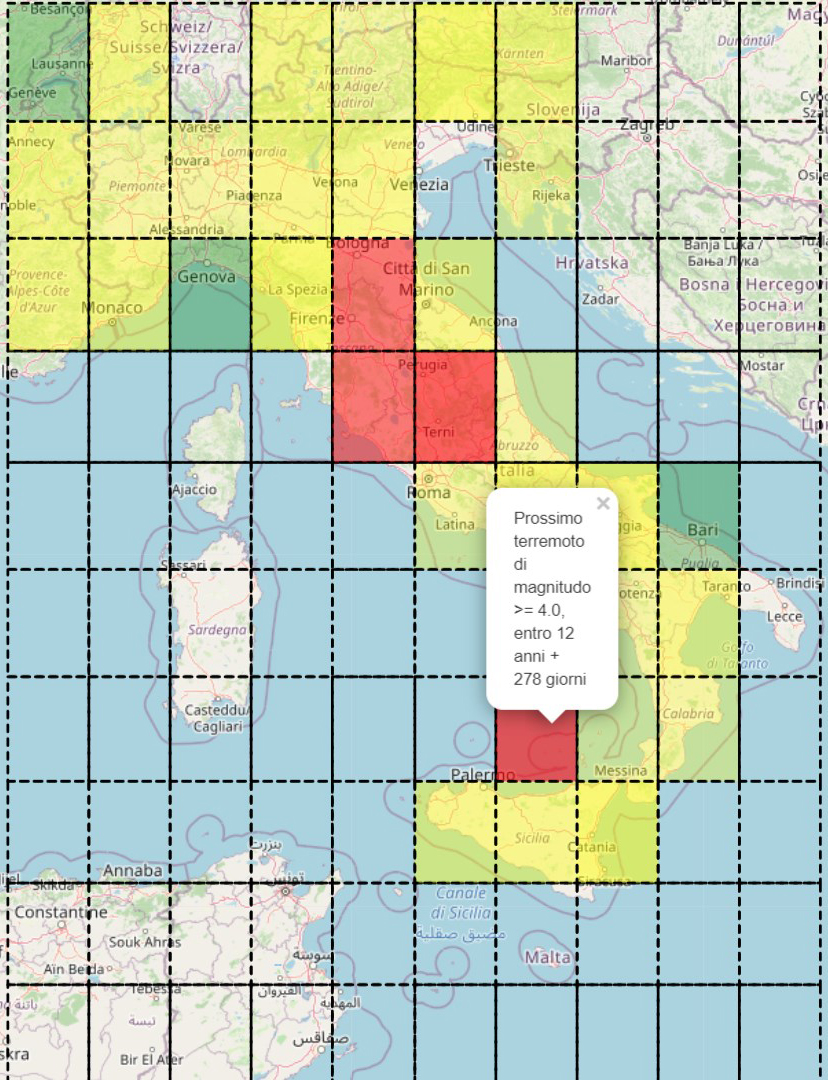
\includegraphics[width=0.600\textwidth]{images/10x10_mag4_12anniEvidenziato_CPTI15.jpg}
   \caption{Griglia 10x10 con DB CPTI15, magnitudo minima 4 evidenziata la cella con previsione pi\`u vicina}
   \label{fig:10x10_mag4_12anniEvidenziato}
\end{figure}

La prima che voglio analizzare \`e la Figura \ref{fig:10x10_mag4_12anniEvidenziato} questa \`e prodotta dall'input n = 10, x = 4 quindi avremo una griglia 10x10 che in base al criterio descritto sopra colora la mappa e ne rappresenta una stima in anni, che prevede con probabilit\`a del 75\% tra quanto avverr\`a il prossimo terremoto nella cella i-esima. In questo caso specifico prendiamo la cella colorata di rosso scuro, quella con numero minimo di giorni per i quali \`e previsto un terremoto con magnitudo $\ge$ 4, la cella in questione \`e la 7x7, vediamo come cliccandoci sopra si apre un popup che ci dice fra 12 anni + 278 giorni al massimo avverr\`a il prossimo terremoto con magnitudo $\ge$ 4, ora per verificare se la stima fatta dall'algoritmo ha dato esito positivo andiamo a utilizzare il programma descritto precedentemente che ci permette di verificarlo.

\begin{figure}[H]
   \centering
   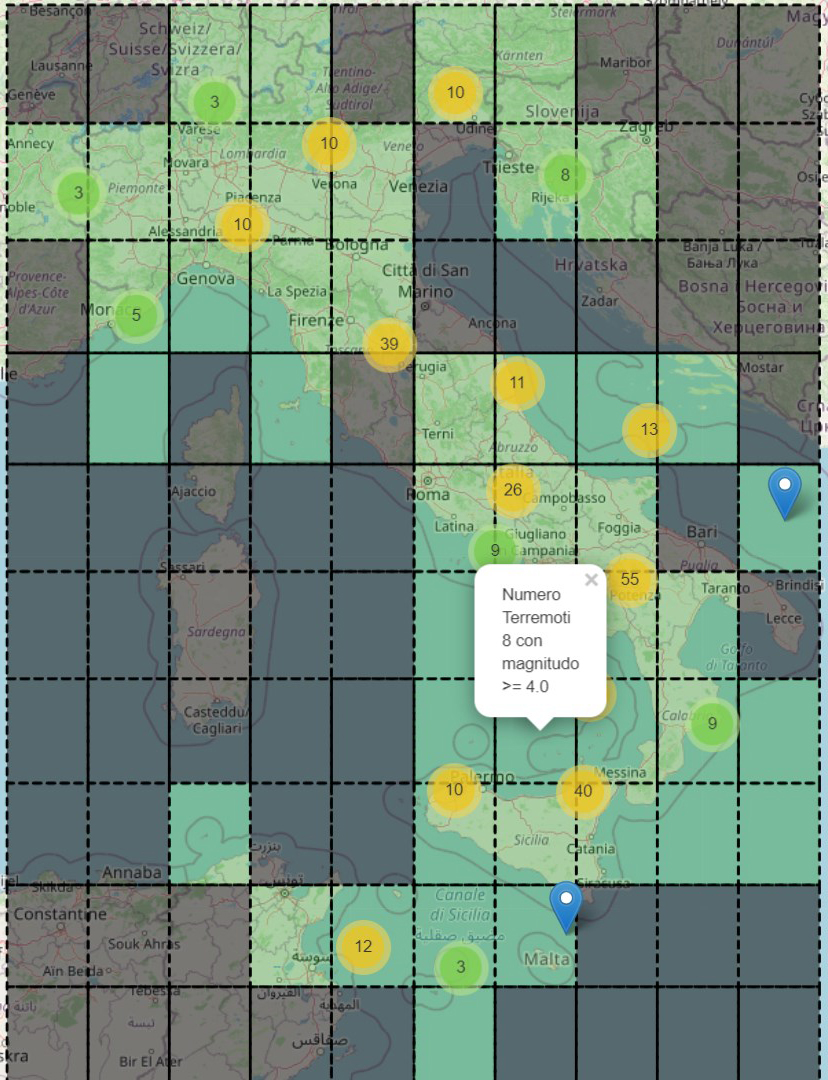
\includegraphics[width=0.600\textwidth]{images/10x10_mag4_12anniDopo_CPTI15.jpg}
   \caption{Griglia 10x10 con DB CPTI15, magnitudo minima 4 terremoti avvenuti dal 1981 al 1993}
   \label{fig:10x10_mag4_12anniDopo}
\end{figure}

Andando a cliccare sulla cella che abbiamo preso in considerazione, scopriamo che dal 1981 al 1993, ovvero nei 12 anni successivi ai dati che ho usato per stimare la previsione, ci sono stati 8 terremoti con magnitudo $\ge$ 4. Quindi l'esito dell'algoritmo \`e stato positivo. Ora voglio portare alla luce un fatto, sulle celle precedentemente colorate di rosso, gi\`a a 12 anni di distanza si sono registrati terremoti tranne che su una la 4x5. Vorrei prendere in analisi proprio questa, vedendo fra quanti anni l'algoritmo stima ci sar\`a il prossimo terremoto al massimo.

\begin{figure}[H]
   \centering
   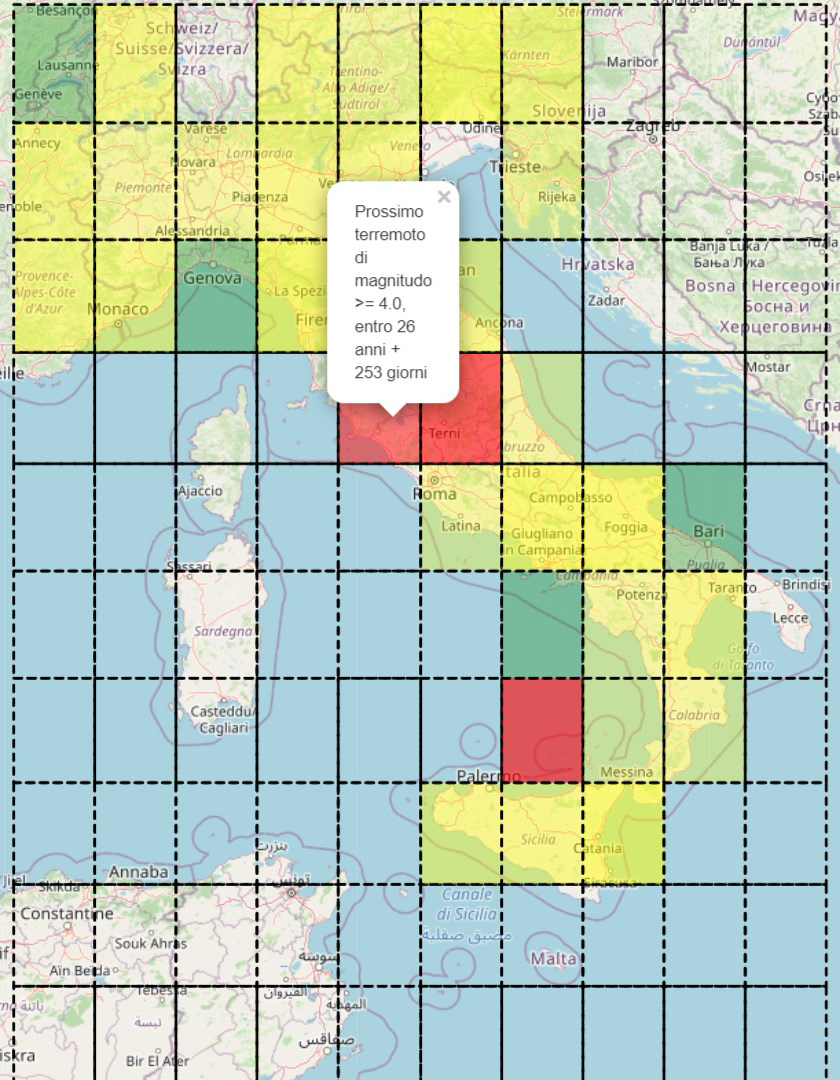
\includegraphics[width=0.600\textwidth]{images/10x10_mag4_26anniEvidenziato_CPTI15.jpg}
   \caption{Griglia 10x10 con DB CPTI15, magnitudo minima 4 evidenziata la cella con previsione subito successiva alla pi\`u vicina}
   \label{fig:10x10_mag4_26anniEvidenziato}
\end{figure}

Come si vede dalla Figura  \ref{fig:10x10_mag4_26anniEvidenziato} nella cella 4x5 la stima minima in anni \`e 26, quindi la griglia risultante del programma che verifica non pu\`o essere presa in considerazione, vado a generare una nuova griglia questa volta aumentando l'intervallo di anni da tenere in considerazione.

\begin{figure}[H]
   \centering
   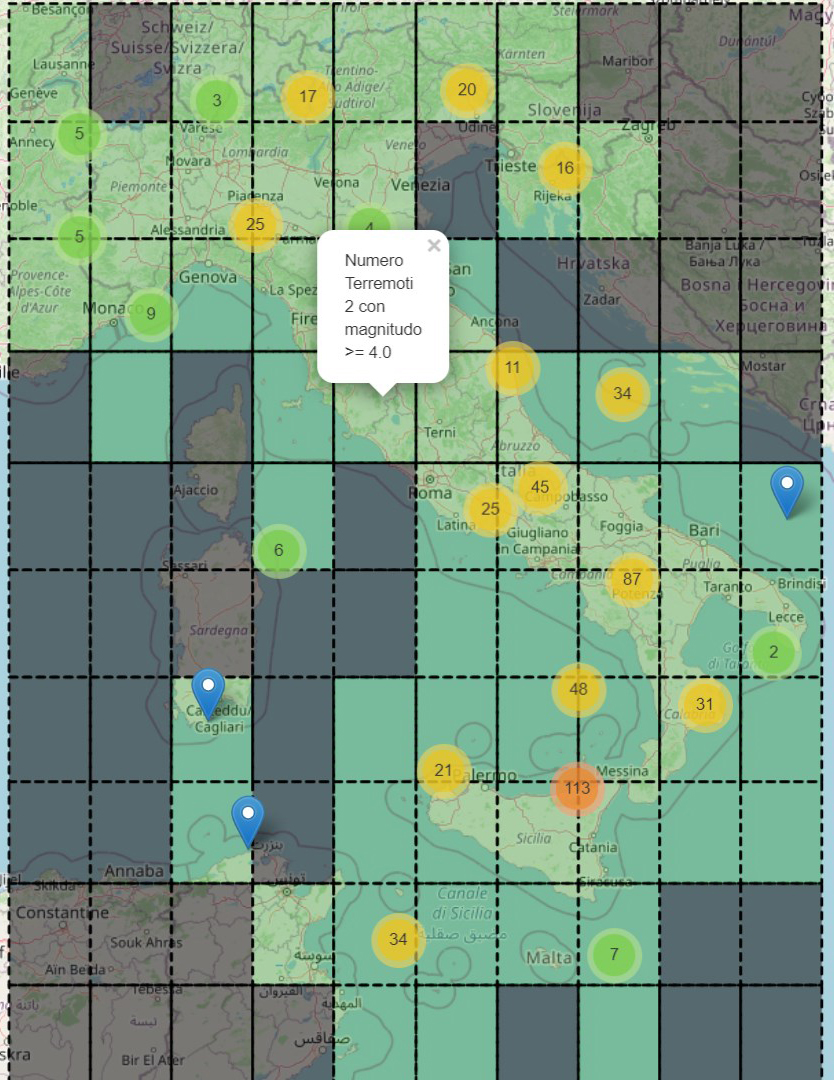
\includegraphics[width=0.600\textwidth]{images/10x10_mag4_26anniDopo_CPTI15.jpg}
   \caption{Griglia 10x10 con DB CPTI15, magnitudo minima 4 terremoti avvenuti dal 1981 al 2007}
   \label{fig:10x10_mag4_26anniDopo}
\end{figure}

La cella 4x5 risulta ora colorata di verde, infatti andando nel dettaglio riusciamo a vedere che dal 1981 al 2007 i terremoti avvenuti sono 2. Anche se il numero \`e piccolo anche questo risultato porta esito positivo dell'algoritmo. Come si vede dalle Figure \ref{fig:10x10_mag4_12anniDopo} e \ref{fig:10x10_mag4_26anniDopo} ci sono celle colorate in verde anche dove l'algoritmo non aveva calcolato una stima, questo avviene perch\'e in quelle celle non erano presenti dati storici o quelli presenti erano insufficienti, e quindi non hanno permesso la creazione della stima. Infatti quando le celle dell'output del programma basato sul secondo approccio sono trasparenti, significa che non ci sono stati pi\`u di 10 terremoti in quella cella superiori alla magnitudo x presa in considerazione, pertanto la stima non viene fatta. Questo evidenzia quanto sia importante avere a disposizione una grande mole di dati per far si che l'algoritmo porti risultati pi\`u precisi. Di seguito mostro graficamente altri esempi andando a prendere in considerazione una magnitudo pi\`u alta, quindi solitamente questo comporta un minor numero di dati storici a disposizione, in quanto terremoti con una magnitudo pi\`u alta avvengono pi\`u raramente (per nostra fortuna).

\begin{figure}[H]
   \centering
   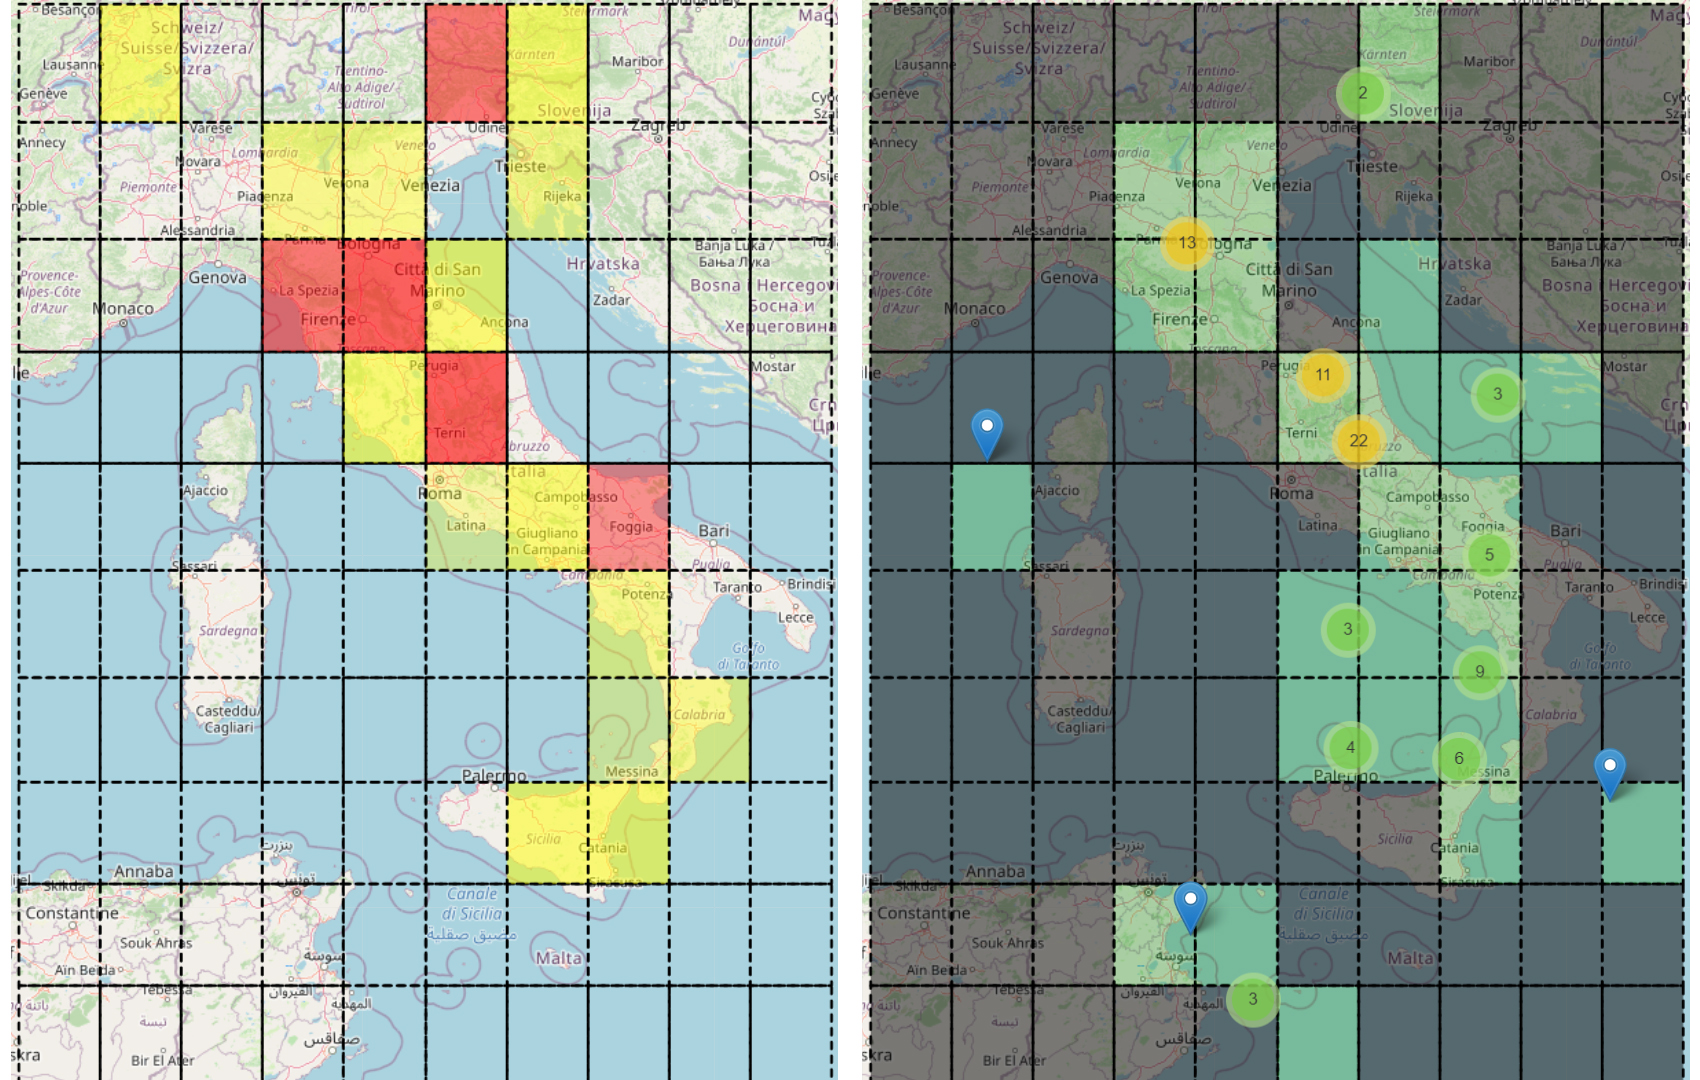
\includegraphics[width=0.835\textwidth]{images/10x10_mag5_confronto_36anniDopo_CPTI15.jpg}
   \caption{Griglia 10x10 con DB CPTI15, magnitudo minima 5, confrontato con terremoti avvenuti dal 1981 al 2017}
   \label{fig:10x10_mag5_36anniDopo}
\end{figure}

La cella con la previsione pi\`u vicina \`e la cella rossa nel centro Italia che riporta una previsione a 41 anni, mentre le celle gialle partono tutte da poco pi\`u di 100 anni, queste sono tutte previsioni a lungo termine, quindi non avendo a disposizione i dati oltre il 2017 posso confrontare la previsione soltanto con i terremoti avvenuti dal 1981 al 2017 che sono quindi i terremoti avvenuti fino a 36 anni dopo i dati utilizzati per la previsione. Come si vede dalla Figura \ref{fig:10x10_mag5_36anniDopo} nelle celle colorate di rosso dopo 36 anni sono gi\`a avvenuti dei sismi, tranne che nella cella 1x6 dove la previsione mi dice 99 anni, quindi \`e una delle rosse pi\`u al limite, ovvero rientra quasi tra le celle gialle che partono da poco pi\`u di 100 anni.\\
Di seguito faccio ulteriori confronti con una griglia pi\`u dettagliata ovvero 15x15.

\begin{figure}[H]
   \centering
   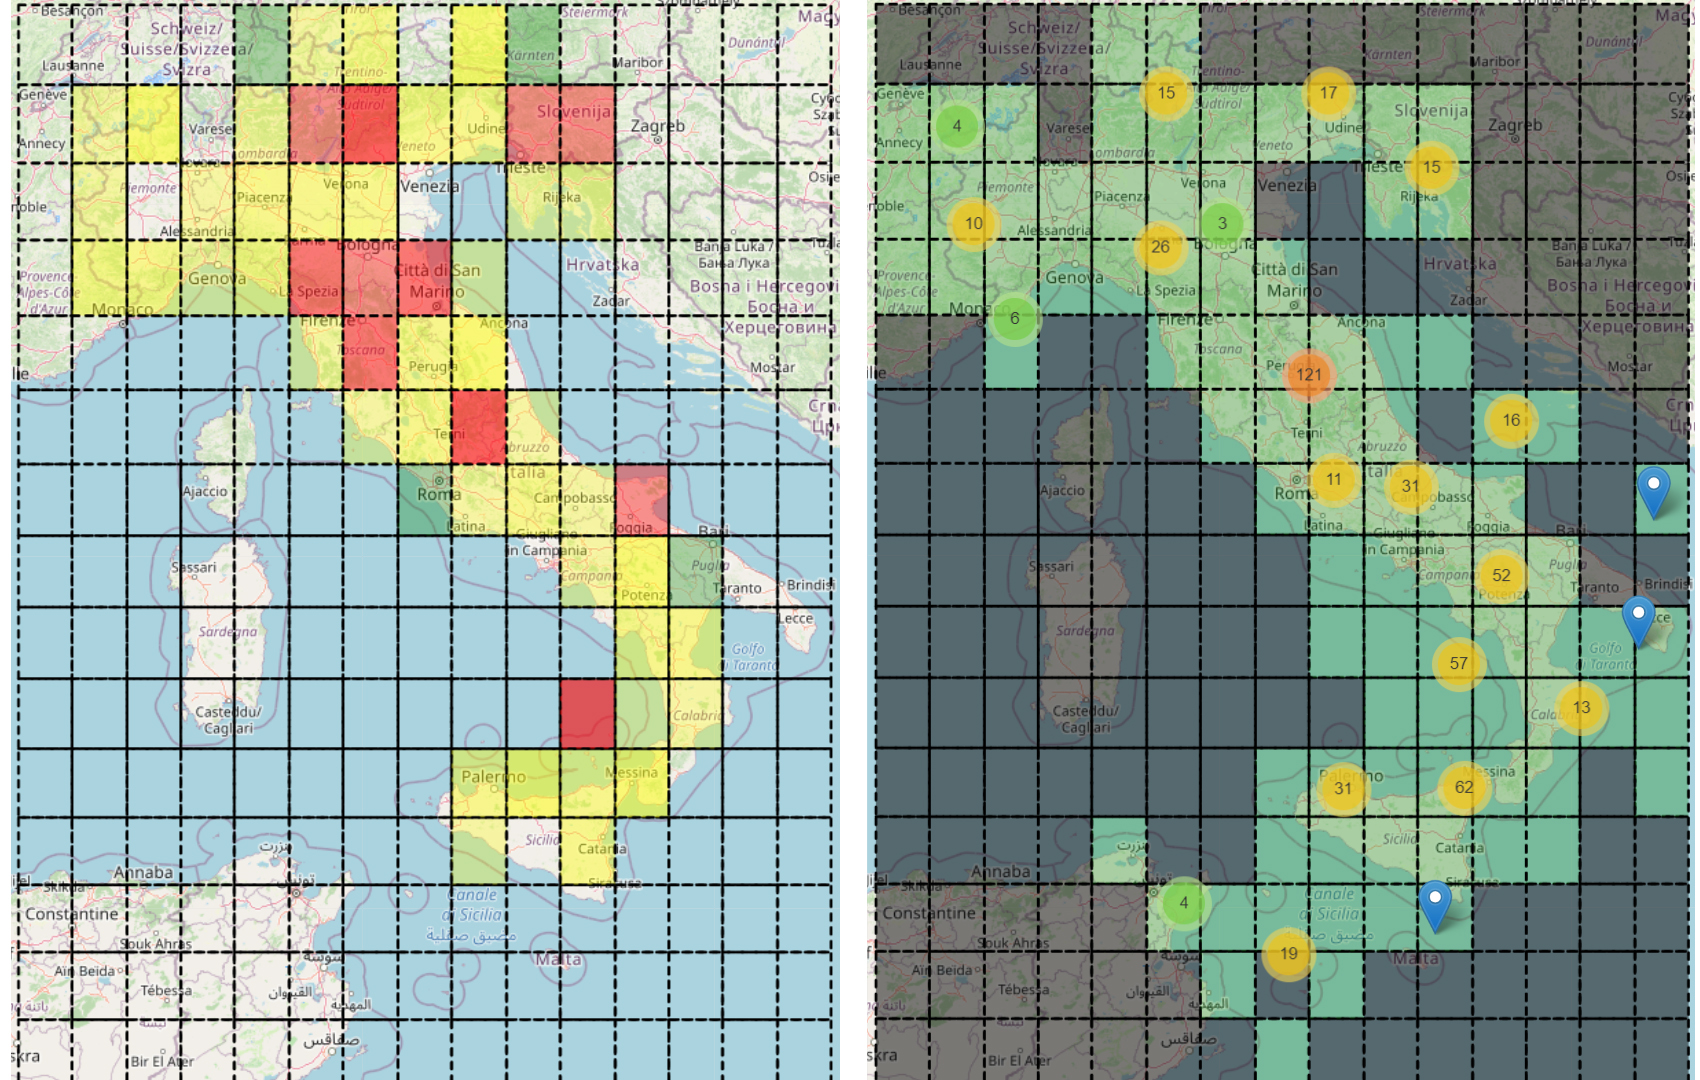
\includegraphics[width=0.835\textwidth]{images/15x15_mag4_confronto_18anniDopo_CPTI15.jpg}
   \caption{Griglia 15x15 con DB CPTI15, magnitudo minima 4, confrontato con terremoti avvenuti dal 1981 al 1999}
   \label{fig:15x15_mag4_18anniDopo}
\end{figure}

\begin{figure}[H]
   \centering
   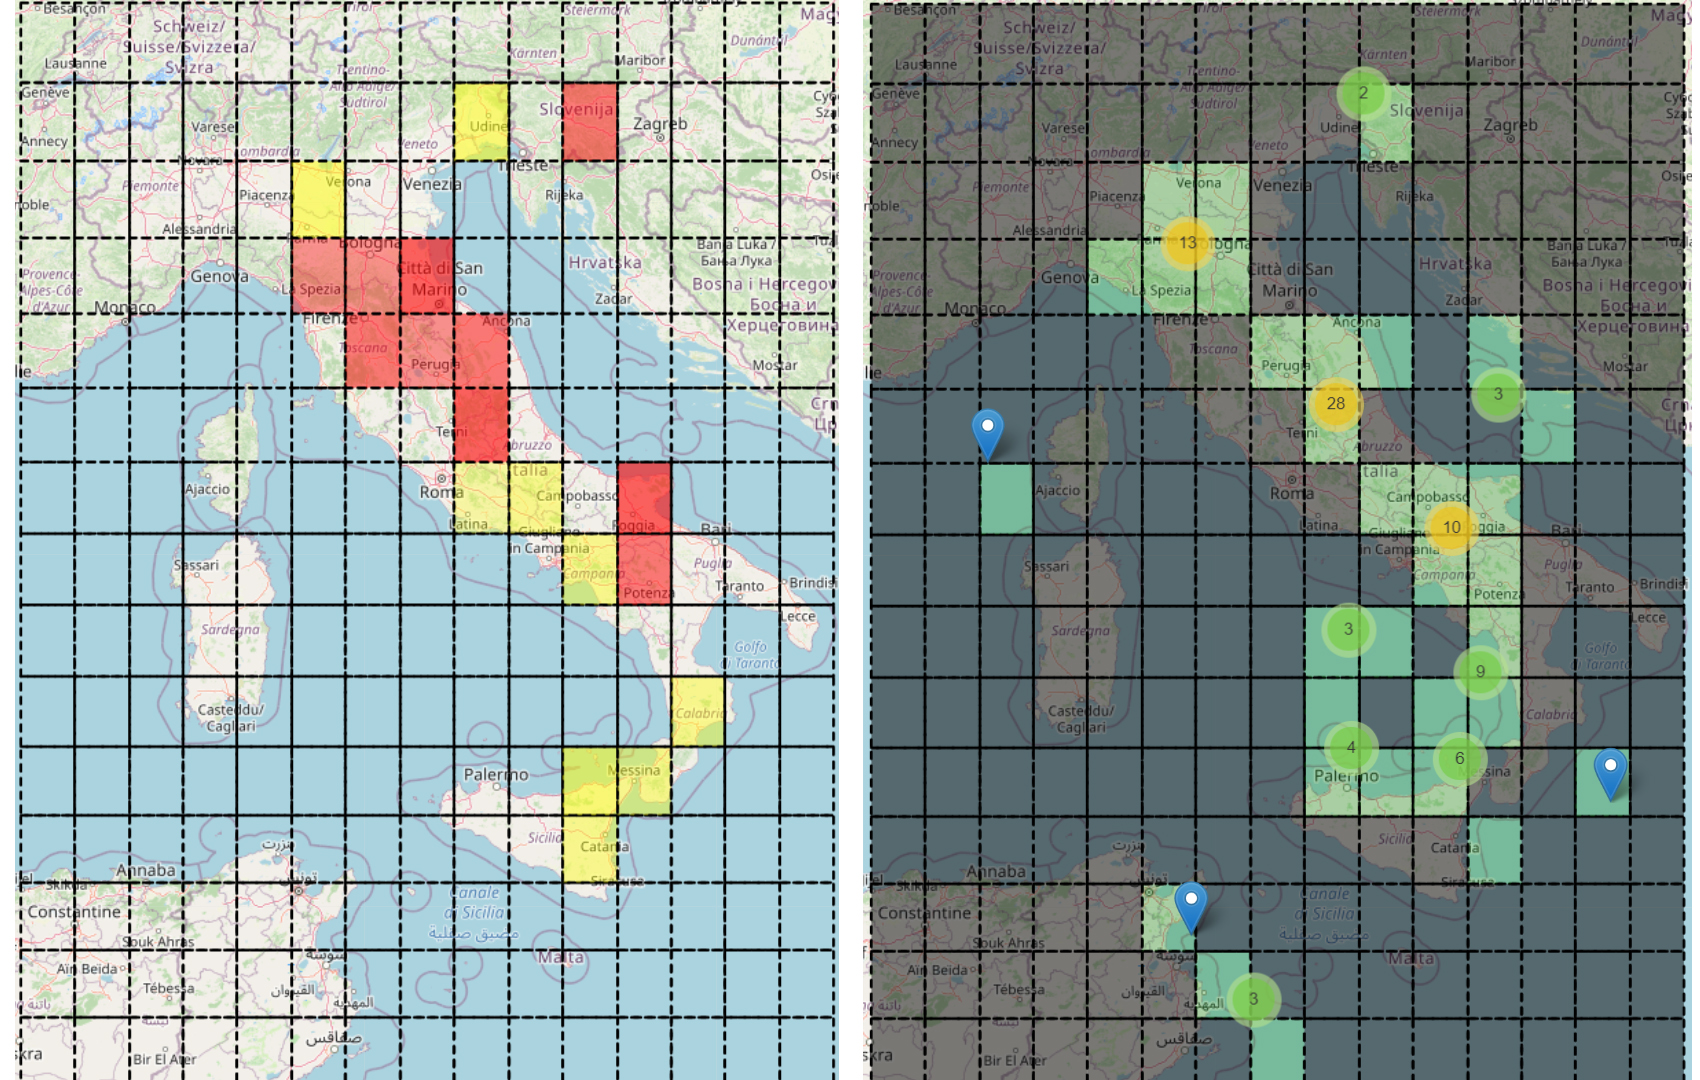
\includegraphics[width=0.835\textwidth]{images/15x15_mag5_confronto_36anniDopo_CPTI15.jpg}
   \caption{Griglia 15x15 con DB CPTI15, magnitudo minima 5, confrontato con terremoti avvenuti dal 1981 al 2017}
   \label{fig:15x15_mag5_36anniDopo}
\end{figure}

Anche in queste due ultime rappresentazioni grafiche dei risultati si vede come l'algoritmo funziona discretamente bene, prevedendo per la maggior parte delle celle i terremoti che avverranno entro una data limite. Nello specifico analizzando la Figura \ref{fig:15x15_mag4_18anniDopo} la cella rossa nel centro Italia \`e quella con la previsione pi\`u vicina, ovvero 18 anni a partire dal 1980, mentre le altre due subito successive, colorate di rosso scuro sono quelle nel nord e nel sud Italia, che rispettivamente hanno una previsione di 24 e 22 anni, in questo caso ho voluto confrontare con la mappa riportante i terremoti avvenuti dal 1981 al 1999 quindi prendendo come riferimento la cella nel centro Italia, e come si vede dalla foto l'esito per quella cella \`e stato positivo essendo avvenuti ben 44 terremoti di magnitudo $\ge$ 4. Anche per le altre due celle rosse gi\`a 18 anni dopo troviamo dei terremoti avvenuti in esse, e non solo, molte delle celle gialle sono state gi\`a colpite da terremoti con magnitudo $\ge$ 4 entro 18 anni. Per la Figura \ref{fig:15x15_mag5_36anniDopo} non entro nel dettaglio in quanto la previsione minima nella cella rosso scuro del centro Italia supera i 50 anni e la mappa di confronto come anche detto in precedenza non pu\`o superare i 36 anni, quindi lascio parlare la rappresentazione grafica.\\
Ometto l'analisi numerica dei risultati, in quanto risulterebbe scorretto affermare l'affidabilit\`a dell'algoritmo predittivo soltanto con i dati a disposizione, questo perch\'e la maggior parte delle celle nelle mappe in output dell'algoritmo, vanno fuori dal range nel quale \`e possibile fare verifiche con i dati a disposizione, quindi mi attengo al fatto di aver usato la formula derivante dalla disuguaglianza di Chebychev, pertanto a priori se come gi\`a detto, considero le rilevazioni empiriche sul passato assumendo che l'intervallo di tempo che intercorre fra due terremoti si comporti come una variabile aleatoria, posso affermare che il prossimo terremoto avverr\`a nella cella i-esima entro il numero di anni previsti dall'algoritmo con una probabilit\`a del 75\%.

\section{Strumenti utilizzati}\label{analisiDati}

Per analizzare i dati ho creato un programma scritto in linguaggio Python, linguaggio dinamico, semplice e flessibile che supporta la programmazione ad oggetti, strutturata e funzionale. Uno dei punti di forza di questo linguaggio \`e il poter importare una serie di librerie, ognuna delle quali pensata per uno specifico scopo di applicazione. Nel mio progetto saranno due le librerie che faranno da pilastri del programma:
\begin{itemize}
    \item \textit{Pandas} - La prima libreria essenziale ai fini del mio lavoro \`e un software scritto in linguaggio Python utilizzato per la manipolazione e l'analisi di grandi quantit\`a di dati, permette pertanto di leggere svariati formati con i quali solitamente si immagazzinano dati in formato digitale. Il formato messo a disposizione dalla maggior parte degli enti che immagazzinano dati riguardanti i terremoti (e non), come anche l'INGV, sono in formato .csv. Questo formato pu\`o essere immaginato (da noi persone) come una tabella, dove nella prima riga troviamo l'intestazione di ogni campo, per riconoscere i valori memorizzati nelle righe successive, ma per essere di facile comprensione per ogni programma i dati sono organizzati nella seguente maniera: suddivisi in righe, ogni riga utilizza una virgola come carattere di separazione tra un valore e il successivo e la prima riga contiene l'intestazione, ovvero il nome, dei valori rappresentati nelle righe successive;
    \item \textit{Folium} - I dati sarebbero inutili se non ci poniamo l'obiettivo di rappresentarli e visualizzarli al meglio, per rispondere a ci\`o nasce questa libreria. Nel mio caso \`e stata utile per l'analisi visiva geospaziale dei dati, ovvero per la creazione di una mappa interattiva. Questo utilizzo \`e reso possibile grazie all'interazione tra \textit{Folium} e la famosa libreria \textit{Leaflet}\footnote{\`E la principale libreria JavaScript open source per mappe interattive ottimizzate per dispositivi mobili.}.
\end{itemize}